\section{状态分布与首次到达问题}
\label{sec:ctsp-distributions}

上一节逐路径地求解方程：给定一条噪声路径，得到一条状态路径。很多问题并不关心某一条路径，而关心整体规律：某个时刻状态落在哪里的概率，从某处出发最终获得的平均收益，先碰到哪一侧边界的概率，平均要等多久。本节说明，这些量都满足确定性的方程。桥梁是Itô公式中的漂移部分，即生成元；它把随机路径上的平均变成偏微分方程或常微分方程，使第~\ref{chap:partial-differential-equations}章的方法获得概率解释，也让概率方法反过来给出这些方程的解。

\subsection{生成元与测试函数期望}
\label{sec:ctsp-generator-dynkin}

\paragraph{从Itô公式读出生成元}
考虑自治的Itô扩散$\mathrm d\bm X_t=\bm b(\bm X_t)\,\mathrm dt+\bm\sigma(\bm X_t)\,\mathrm d\bm W_t$，记扩散矩阵$\bm a=\bm\sigma\bm\sigma^\top$。对$f\in C^2_c(\mathbb R^d)$（二阶连续可微且支撑有界），Itô公式给出
\[
  f(\bm X_t)=f(\bm X_0)+\int_0^t\mathcal Lf(\bm X_s)\,\mathrm ds+\int_0^t\nabla f(\bm X_s)^\top\bm\sigma(\bm X_s)\,\mathrm d\bm W_s ,
\]
其中$\mathcal L$是式~\eqref{eq:ctsp-diffusion-generator}中的二阶微分算子
\begin{equation}
  \mathcal Lf=\sum_ib_i\partial_if+\frac12\sum_{i,j}a_{i,j}\partial_i\partial_jf .
  \label{eq:ctsp-generator-explicit}
\end{equation}
若系数连续，$f$的支撑有界保证随机积分的被积过程有界，它是真鞅；取期望、除以$t$并令$t\downarrow0$，得到$\lim_{t\downarrow0}t^{-1}(\mathbb E_{\bm x}f(\bm X_t)-f(\bm x))=\mathcal Lf(\bm x)$。所以$\mathcal L$正是第~\ref{sec:ctsp-semigroup}节意义下生成元在$C^2_c$上的作用：漂移贡献一阶项，扩散贡献二阶项。

不同驱动在生成元中留下不同形式的项。方程中含有跳跃$\bm\gamma(\bm X_{t-})\,\mathrm dN_t$时，跳跃Itô公式~\eqref{eq:ctsp-jump-ito}在漂移中多出$\lambda[f(\bm x+\bm\gamma(\bm x))-f(\bm x)]$，生成元多了一个有限差项。纯跳跃的连续时间Markov链只有这种项，$\mathcal Lf(i)=\sum_jq_{i,j}[f(j)-f(i)]$，即生成矩阵作用于向量$f$。三种情形放在一起：漂移推动，扩散抹平，跳跃搬运。

\paragraph{Dynkin公式}
在随机时刻停止后，Itô公式的期望形式仍然成立，但需要条件来保证随机积分在停止后的期望为零。

\begin{theorem}[Dynkin公式]
  \label{thm:ctsp-dynkin}
  设$\bm b,\bm\sigma$连续，方程从$\bm x$出发有不爆炸的解。设$f\in C^2(\mathbb R^d)$，$\tau$是停时且$\mathbb E_{\bm x}\tau<\infty$，并且存在有界集合$D$，使停止前$\bm X_t\in D$（或$f$支撑有界）。则
  \begin{equation}
    \mathbb E_{\bm x}f(\bm X_\tau)=f(\bm x)+\mathbb E_{\bm x}\int_0^\tau\mathcal Lf(\bm X_s)\,\mathrm ds .
    \label{eq:ctsp-dynkin}
  \end{equation}
  对$V\in C^{2,1}$，同样的条件下有$\mathbb E_{\bm x}V(\tau,\bm X_\tau)=V(0,\bm x)+\mathbb E_{\bm x}\int_0^\tau(\partial_s+\mathcal L)V(s,\bm X_s)\,\mathrm ds$。
\end{theorem}

\begin{proof}
在$D$的闭包上，$\nabla f^\top\bm\sigma$与$\mathcal Lf$连续因而有界。停止在$\tau\wedge n$，随机积分的被积过程有界，期望为零，于是$\mathbb E_{\bm x}f(\bm X_{\tau\wedge n})=f(\bm x)+\mathbb E_{\bm x}\int_0^{\tau\wedge n}\mathcal Lf(\bm X_s)\,\mathrm ds$。令$n\to\infty$：左端由路径连续与$f$在$\bar D$上有界，用控制收敛；右端被积函数被$\sup_{\bar D}|\mathcal Lf|\cdot\tau$控制，而$\mathbb E\tau<\infty$。含时间的版本只需把Itô公式换成定理~\ref{thm:ctsp-ito-formula}的含时间形式。
\end{proof}

式~\eqref{eq:ctsp-dynkin}称为\term{Dynkin公式}（Dynkin formula）。条件各有用途：$\mathbb E\tau<\infty$保证时间积分可积，状态限制在有界集合中保证函数及其导数有界，从而局部鞅确实是零均值的鞅。去掉其中任一条，等式可能失败；第~\ref{sec:ctsp-optional-sampling}节的首次到达时刻$\tau_a$就是$f(x)=x$、$\mathcal Lf=0$而等式失败的例子，那里$\mathbb E\tau_a=\infty$，路径也不受界。

\paragraph{弱形式的分布演化}
取$\tau=t$为固定时刻，Dynkin公式变成关于状态分布的等式。记$\mu_t$为$\bm X_t$的分布，对$f\in C^2_c$，
\begin{equation}
  \int f\,\mathrm d\mu_t-\int f\,\mathrm d\mu_0=\int_0^t\int\mathcal Lf\,\mathrm d\mu_s\,\mathrm ds .
  \label{eq:ctsp-weak-evolution}
\end{equation}
这个等式不要求$\mu_t$有密度：初值是点质量、扩散退化、或者状态空间是离散的，它都成立。它的含义是，每一个光滑的“读数”$f$，其平均值的变化率等于$\mathcal Lf$的平均值。

反过来问：若一族分布对所有$f\in C^2_c$满足式~\eqref{eq:ctsp-weak-evolution}，或更强地，若过程使$f(\bm X_t)-\int_0^t\mathcal Lf(\bm X_s)\,\mathrm ds$对所有$f\in C^2_c$都是鞅，能否推出过程的规律就是这个方程的解？这称为\term{鞅问题}（martingale problem）。当鞅问题适定，即这样的规律存在且唯一时，答案是肯定的；例如系数有界连续且$\bm a$一致正定时鞅问题适定\scite{math-kallenberg2021probability}。这说明第~\ref{sec:ctsp-semigroup}节的抽象生成元与本节的微分算子之间还隔着一层验证：随机方程给出一个具体的候选生成元，过程的规律是否被它唯一确定，取决于定义域与适定性。

\subsection{后向方程与密度演化}
\label{sec:ctsp-backward-forward}

\paragraph{后向方程：固定终点的平均收益}
设在终点$T$获得收益$g(\bm X_T)$，问从时刻$t$、状态$\bm x$出发的平均收益
\begin{equation}
  u(t,\bm x)=\mathbb E\bigl[g(\bm X_T)\bigm|\bm X_t=\bm x\bigr]
  \label{eq:ctsp-backward-value}
\end{equation}
满足什么方程。这个量对每个起点都要算，用偏微分方程描述它最自然。

关键观察是：沿着路径，$u(t,\bm X_t)=\mathbb E[g(\bm X_T)\mid\mathcal F_t]$（由Markov性质），所以它是一个鞅。若$u\in C^{2,1}$，含时间的Itô公式给出
\[
  \mathrm du(t,\bm X_t)=(\partial_t u+\mathcal Lu)(t,\bm X_t)\,\mathrm dt+\nabla u^\top\bm\sigma\,\mathrm d\bm W_t .
\]
一个连续鞅如果同时是有限变差过程与局部鞅之和，有限变差部分必须为零，于是漂移$(\partial_tu+\mathcal Lu)(t,\bm X_t)$沿路径恒为零。在扩散非退化、状态能到达各处时，这推出
\begin{equation}
  \partial_tu+\mathcal Lu=0,\qquad u(T,\bm x)=g(\bm x),
  \label{eq:ctsp-backward-equation}
\end{equation}
称为后向方程：它从终点条件出发，沿时间向回求解。

上面的推导假设$u$足够光滑，这需要单独论证。实际中更常用的是反方向的验证：若已经找到$u\in C^{2,1}$满足式~\eqref{eq:ctsp-backward-equation}，并且$\nabla u^\top\bm\sigma$满足使随机积分为真鞅的可积条件，那么由Itô公式，$u(s,\bm X_s)$在$[t,T]$上是鞅，比较两端取值即得$u(t,\bm x)=\mathbb E[g(\bm X_T)\mid\bm X_t=\bm x]$。这一论证完全依赖含时间的Itô公式：要验证的是$V(t,\bm X_t)$的漂移为零，而$V$同时依赖时间和状态。

\begin{example}[Brownian运动与热方程]
  \label{ex:ctsp-heat-equation}
  对Brownian运动，$\mathcal L=\frac12\partial_{xx}$，后向方程是$\partial_tu+\frac12\partial_{xx}u=0$，即时间反向的热方程。取$g(x)=x^2$，$u(t,x)=\mathbb E[(x+W_T-W_t)^2]=x^2+(T-t)$，直接核对$\partial_tu+\frac12\partial_{xx}u=-1+1=0$。一般地，$u(t,x)=\int g(y)p_{T-t}(x,y)\,\mathrm dy$，其中$p$是式~\eqref{eq:ctsp-heat-kernel}的热核；这正是第~\ref{chap:partial-differential-equations}章用热核表示的热方程解，只是这里把热核读作转移密度，把解读作平均收益。
\end{example}

\paragraph{前向方程：分布的流动}
后向方程关心“从哪里出发”，以出发状态为变量；前向方程关心“流到哪里”，以到达状态为变量。若$\mu_t$对Lebesgue测度有密度$p(t,\bm x)$，把弱形式~\eqref{eq:ctsp-weak-evolution}中的导数通过分部积分从$f$移到$p$上：漂移项分部积分一次，扩散项两次。测试函数支撑有界，边界项消失，得到
\[
  \int f\,\partial_tp\,\mathrm d\bm x=\int f\Bigl[-\sum_i\partial_i(b_ip)+\frac12\sum_{i,j}\partial_i\partial_j(a_{i,j}p)\Bigr]\mathrm d\bm x .
\]
对所有$f\in C^2_c$成立，所以在分布意义下
\begin{equation}
  \partial_tp=-\sum_i\partial_i(b_ip)+\frac12\sum_{i,j}\partial_i\partial_j(a_{i,j}p),
  \label{eq:ctsp-fokker-planck}
\end{equation}
这就是\term{Fokker--Planck方程}，也称前向Kolmogorov方程。右端的算子是$\mathcal L$的形式伴随$\mathcal L^*$。

把右端写成散度形式$\partial_tp=-\nabla\cdot\bm J$，其中概率流$J_i=b_ip-\frac12\sum_j\partial_j(a_{i,j}p)$，方程就是一条守恒律：某处密度的增减等于概率流的净流入。对全空间积分并假设概率流在无穷远处足够快地消失，得到$\frac{\mathrm d}{\mathrm dt}\int p\,\mathrm d\bm x=0$，总质量守恒。有界区域上的模型还需要边界条件：反射边界要求法向概率流为零，吸收边界要求边界上密度为零，后者使区域内的总质量随时间减少。

\begin{example}[OU密度的流动]
  \label{ex:ctsp-ou-density}
  对$\mathrm dX=-\lambda X\,\mathrm dt+\sigma\,\mathrm dW$，Fokker--Planck方程为$\partial_tp=\partial_x(\lambda xp)+\frac{\sigma^2}2\partial_{xx}p$。从$x_0$出发，由第~\ref{sec:ctsp-linear-sde}节的显式解，$p(t,\cdot)$是$\mathcal N(x_0e^{-\lambda t},\sigma^2(1-e^{-2\lambda t})/(2\lambda))$的密度，可以逐项代入核对。令$\partial_tp=0$并要求概率流为零，$\lambda xp+\frac{\sigma^2}2p'=0$，解得稳态密度$p\propto\exp\{-\lambda x^2/\sigma^2\}$，即$\mathcal N(0,\sigma^2/(2\lambda))$。图~\ref{fig:ctsp-fokker-planck-snapshots}画出$\lambda=1,\sigma=1,x_0=3$时的几个时间截面：起初是集中在$3$附近的窄峰，随后峰顶向左漂移、宽度增加，最后停在稳态上。
\end{example}

\begin{figure}[htbp]
  \centering
  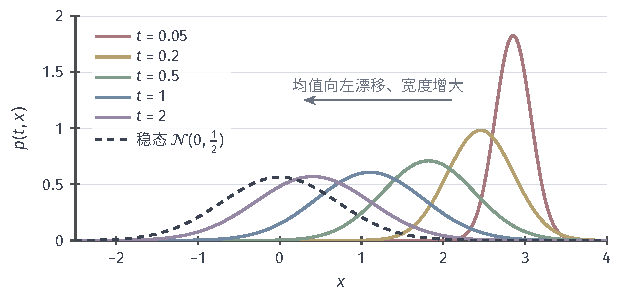
\includegraphics[width=105mm]{figures/03-optimization-evolution-and-signals/02-processes-and-trajectory-evolution/tikz/ctsp-fokker-planck-snapshots/figure.pdf}
  \caption{Fokker--Planck方程的时间截面（解析解，无模拟）。模型为$\mathrm dX=-X\,\mathrm dt+\mathrm dW$，从$x_0=3$出发，$p(t,\cdot)=\mathcal N(3e^{-t},(1-e^{-2t})/2)$。各色曲线为$t=0.05,0.2,0.5,1,2$的密度，黑虚线为稳态$\mathcal N(0,\frac12)$。漂移把概率质量向原点搬运，扩散把它摊开，二者在稳态处平衡。}
  \label{fig:ctsp-fokker-planck-snapshots}
\end{figure}

\paragraph{两个方程的对偶与适用条件}
后向方程与前向方程是同一个演化的两种描述。设$u$解后向方程，$p$解前向方程，则$\frac{\mathrm d}{\mathrm dt}\int u(t,\bm x)p(t,\bm x)\,\mathrm d\bm x=\int(\partial_tu\,p+u\,\partial_tp)\,\mathrm d\bm x=\int(-\mathcal Lu\cdot p+u\cdot\mathcal L^*p)\,\mathrm d\bm x=0$。也就是说$\mathbb Eu(t,\bm X_t)$与$t$无关，在$t=T$处等于$\mathbb Eg(\bm X_T)$。

从弱形式到式~\eqref{eq:ctsp-fokker-planck}的逐点形式，需要密度存在并且足够光滑，系数也要可微。系数光滑有界、并且扩散\term{一致椭圆}（uniformly elliptic），即$\bm a\succeq c\bm I$对某个常数$c>0$成立，是保证正时刻光滑密度的一组常用充分条件。扩散退化时，概率可以停留在低维集合上，例如第~\ref{sec:ctsp-linear-sde}节的阻尼振子只有速度方向直接受噪声，此时密度是否存在要靠漂移把噪声传到其他方向；无法保证时，应停留在弱形式~\eqref{eq:ctsp-weak-evolution}上。有跳跃时，前向方程中还要加入积分项$\lambda\bigl[\text{跳入}\bm x\text{的质量}-p(t,\bm x)\bigr]$，形式取决于跳幅映射。

\subsection{首次到达与随机表示}
\label{sec:ctsp-first-passage}

\paragraph{退出概率与平均退出时间}
设$D\subseteq\mathbb R^d$是有界开区域，$\tau=\inf\{t:\bm X_t\notin D\}$是首次退出时刻。两个典型问题是：从$\bm x$出发，退出时落在边界某一部分$\Gamma$上的概率$u(\bm x)=\mathbb P_{\bm x}(\bm X_\tau\in\Gamma)$，以及平均退出时间$v(\bm x)=\mathbb E_{\bm x}\tau$。

Dynkin公式把它们化为边值问题。设$u\in C^2(D)\cap C(\bar D)$满足
\begin{equation}
  \mathcal Lu=0\ \text{于}D,\qquad u=g\ \text{于}\partial D ,
  \label{eq:ctsp-exit-bvp}
\end{equation}
其中$g$为边界上的给定函数（求退出概率时取$g=\mathbb I_\Gamma$），并且$\mathbb E_{\bm x}\tau<\infty$。对$u$在稍小的区域上使用Dynkin公式，再让区域扩大到$D$，得到$u(\bm x)=\mathbb E_{\bm x}g(\bm X_\tau)$。同样，若$v$满足$\mathcal Lv=-1$于$D$、$v=0$于$\partial D$，则$\mathbb E_{\bm x}\tau=v(\bm x)$：Dynkin公式中的时间积分恰好累计出$\tau$本身。

推导中每个条件都承担具体作用。$\mathbb E_{\bm x}\tau<\infty$保证过程确实会离开并使时间积分可积；当扩散一致椭圆、$D$有界时它成立。$u$在$\bar D$上连续保证边界值确实被取到，这需要边界正则：在非正则的边界点，路径可能贴近边界而不立即离开。$u\in C^2(D)$保证可以使用Itô公式。

\begin{example}[区间上的Brownian运动]
  \label{ex:ctsp-bm-exit-ode}
  $D=(0,1)$，$\mathcal L=\frac12\frac{\mathrm d^2}{\mathrm dx^2}$。退出于$1$的概率满足$\frac12u''=0$、$u(0)=0$、$u(1)=1$，所以$u(x)=x$；平均退出时间满足$\frac12v''=-1$、$v(0)=v(1)=0$，所以$v(x)=x(1-x)$。这与第~\ref{sec:ctsp-optional-sampling}节用鞅算出的式~\eqref{eq:ctsp-exit-probability}、\eqref{eq:ctsp-exit-time}一致：那里构造的两个鞅$X_t$与$X_t^2-t$，正是$\mathcal Lu=0$与$\mathcal Lv=-1$的解沿路径的形式。图~\ref{fig:ctsp-exit-problem}用模拟核对了两个函数。
\end{example}

\begin{figure}[htbp]
  \centering
  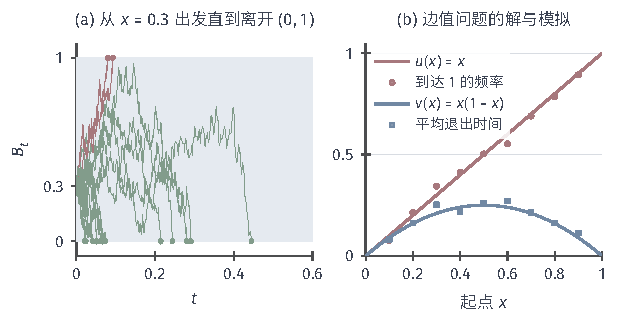
\includegraphics[width=104.5mm]{figures/03-optimization-evolution-and-signals/02-processes-and-trajectory-evolution/tikz/ctsp-exit-problem/figure.pdf}
  \caption{Brownian运动退出区间$(0,1)$。(a)从$x=0.3$出发的$14$条路径，直到离开浅蓝色区域，红色先到达$1$，绿色先到达$0$，圆点为退出位置，为显示只画到$t=0.6$；(b)边值问题的解$u(x)=x$（退出于$1$的概率）与$v(x)=x(1-x)$（平均退出时间），点为每个起点$300$条模拟路径的频率与平均。模拟用步长$2\times10^{-4}$的高斯随机游走并在网格上检测退出，固定随机种子；离散检测会略微推迟退出，平均退出时间因此略有偏高。}
  \label{fig:ctsp-exit-problem}
\end{figure}

加入漂移后，退出概率不再是线性函数。设$\mathrm dX=\mu\,\mathrm dt+\mathrm dW$，$\mu\neq0$，在$(0,1)$中求$u$：方程$\frac12u''+\mu u'=0$的通解为$u=c_1+c_2e^{-2\mu x}$，由边界条件
\[
  \mathbb P_x(\text{先到达}1)=\frac{1-e^{-2\mu x}}{1-e^{-2\mu}} .
\]
$\mu>0$时曲线向上凸起：即使从左端附近出发，向右的漂移也使到达右端的机会显著增加。$\mu\to0$时它回到线性函数$x$。

\paragraph{Feynman--Kac表示}
后向方程可以推广到带“折损”和“流量”的情形。设想沿路径累计收益：在状态$\bm x$处每单位时间获得$f(\bm x)$，同时收益按速率$V(\bm x)\geq0$贴现或衰减，终点再获得$g(\bm X_T)$。

\begin{theorem}[Feynman--Kac表示]
  \label{thm:ctsp-feynman-kac}
  设$\bm b,\bm\sigma$满足定理~\ref{thm:ctsp-sde-existence}的条件，$V\geq0$、$f$、$g$连续有界。若$u\in C^{2,1}([0,T)\times\mathbb R^d)\cap C([0,T]\times\mathbb R^d)$有界，满足
  \begin{equation}
    \partial_tu+\mathcal Lu-Vu+f=0,\qquad u(T,\cdot)=g ,
    \label{eq:ctsp-feynman-kac-pde}
  \end{equation}
  并且$\nabla u^\top\bm\sigma$在每个$[0,T']\times\mathbb R^d$（$T'<T$）上有界，则
  \begin{equation}
    u(t,\bm x)=\mathbb E_{t,\bm x}\Bigl[\int_t^Te^{-\int_t^sV(\bm X_r)\,\mathrm dr}f(\bm X_s)\,\mathrm ds+e^{-\int_t^TV(\bm X_r)\,\mathrm dr}g(\bm X_T)\Bigr].
    \label{eq:ctsp-feynman-kac}
  \end{equation}
\end{theorem}

\begin{proof}
令$E_s=\exp\{-\int_t^sV(\bm X_r)\,\mathrm dr\}$，它是有限变差过程，$\mathrm dE_s=-V(\bm X_s)E_s\,\mathrm ds$，与$u(s,\bm X_s)$的二次协变差为零。由乘积法则与含时间的Itô公式，
\[
  \begin{aligned}
    \mathrm d\bigl[E_su(s,\bm X_s)\bigr]&=E_s\bigl(\partial_su+\mathcal Lu-Vu\bigr)\,\mathrm ds+E_s\nabla u^\top\bm\sigma\,\mathrm d\bm W_s\\
    &=-E_sf(\bm X_s)\,\mathrm ds+E_s\nabla u^\top\bm\sigma\,\mathrm d\bm W_s .
  \end{aligned}
\]
在$[t,T']$上积分，随机积分的被积过程有界，期望为零，于是$u(t,\bm x)=\mathbb E[E_{T'}u(T',\bm X_{T'})+\int_t^{T'}E_sf(\bm X_s)\,\mathrm ds]$。令$T'\uparrow T$，$u$有界连续，$E_s\in(0,1]$，由控制收敛定理得到式~\eqref{eq:ctsp-feynman-kac}。
\end{proof}

式~\eqref{eq:ctsp-feynman-kac}称为\term{Feynman--Kac表示}（Feynman--Kac representation），它有一个直观的读法：$V$是“死亡率”，路径在每段短时间$\mathrm dr$内以概率$V\,\mathrm dr$被杀死，$E_s$就是活到$s$的概率；$f$是存活期间的收益率，$g$是存活到终点的奖励。$V$取常数$r$、$f=0$时，式~\eqref{eq:ctsp-feynman-kac}化为贴现收益$u=e^{-r(T-t)}\mathbb E_{t,\bm x}g(\bm X_T)$。这个表示把偏微分方程的解写成随机路径上的平均，因而可以用模拟路径计算，也可以反过来用PDE的数值方法计算路径期望。

表示的适用范围需要说清。方程中的二阶部分必须是某个扩散的生成元，即扩散矩阵半正定；方程必须是线性的；定理把经典解的存在当作假设，存在性本身要由PDE理论另行保证。超出这些条件的方程，例如非线性方程或对$u$的梯度有非线性依赖的方程，不能直接用Brownian路径的期望表示。
